\section{Programmazione concorrente con OpenMP}\label{capitolo4}
OpenMP è una API multi-piattaforma per il calcolo parallelo a memoria condivisa, essa è disponibile per tutti i sistemi operativi e per i linguaggi C/C++ e Fortran. Questa API si basa su direttive del compilatore, routine di librerie e variabili d'ambiente.\\
Più in dettaglio OpenMP è un'implementazione del multi-threading, nel quale un processo \emph{master} effettua una \emph{fork} e genera un determinato numero di thread \emph{slave} sul quale suddividere il lavoro. Questi thread slave vengono eseguiti concorrentemente su differenti core o processori come mostrato in \ref{fig:openmp}.\\
\begin{figure}
\centering
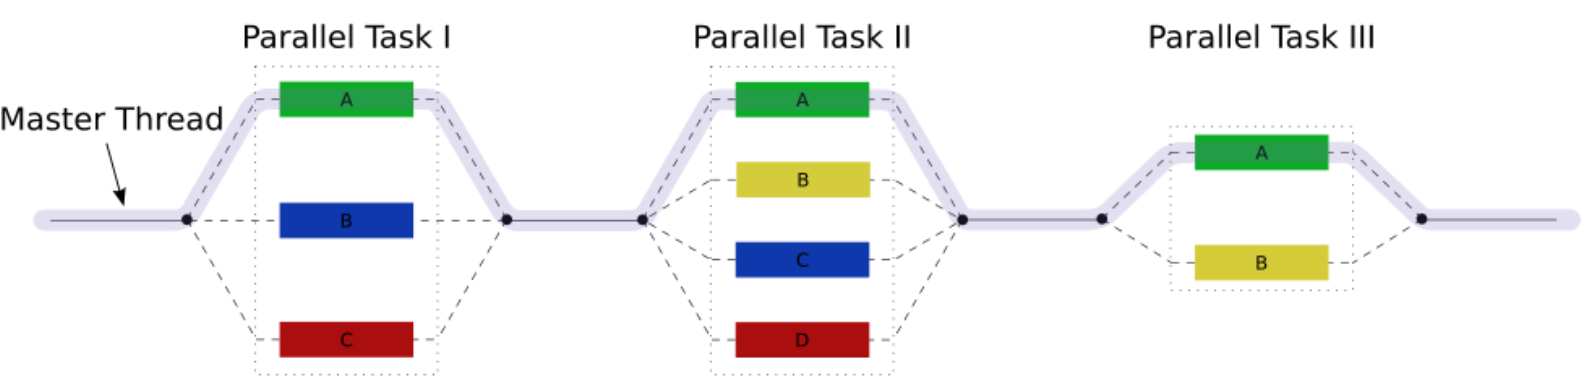
\includegraphics[width=0.7\linewidth]{img/openmp}
\caption{Suddivisione del carico tra diversi threads}
\label{fig:openmp}
\end{figure}
La maggior parte dei costrutti di OpenMP sono direttive del compilatore o \texttt{pragmas}, lo scopo principale dei questa API è quello di parallelizzare i cicli e per farlo offre un approccio incrementale al parallelismo.
Alcune peculiarità sono:
\begin{itemize}
	\item \textbf{Parallelismo innestato:} le API permettono di costruire del thread all'interno di altri thread.
	\item \textbf{Dynamic thread:} le API permettono di cambiare dinamicamente il numero di thread in esecuzione nelle differenti aree parallelizzate.
	\item \textbf{Input/Output: OpenMP} non specifica nulla riguardo agli I/O paralleli è compito del programmatore perciò assicurare la corretta esecuzione parallela.
	\item \textbf{Memory Consistency:} i threads mantengono una loro \emph{cache} e non è quindi necessario mantenere una consistenza con la memoria principale, tuttavia in caso di una variabile condivisa è responsabilità del programmatore assicurare il corretto uso della variabile.
\end{itemize}
Vediamo ora nel Listato \ref{lst:helloopen} un esempio di utilizzo delle API OpenMP
\begin{lstlisting}[language=C++,caption={Esempio di utilizzo delle OpenMP},label=lst:helloopen]
#include <omp.h>
#include <iostream>

using namespace std;
int main () {
	#pragma omp parallel num_threads(3)
	{
		cout<<"Hello World\n"
	}	
}
\end{lstlisting}
Per compilare tale codice è necessario aggiungere l'opzione \texttt{-fopenmp} al normale comando di compilazione.\\
Le direttive OpenMP valide sono identificate dal costrutto
\begin{verbatim}
		#pragma omp name [clause, ...]
\end{verbatim}
dove \emph{name} identifica la direttiva la quale può essere seguita da una o più opzioni. Una delle direttive più importanti è la direttiva \texttt{parallel} senza la quale un programma verrebbe eseguito sequenzialmente. Quando un thread raggiunge la direttiva \texttt{parallel} esso crea una team di  threads ed esso ne diventa il master. A partire dall'inizio della regione parallela il codice viene duplicato e tutti i thread eseguono lo stesso codice. Esiste un \emph{barrier} implicito alla fine della regione parallela dopo il quale solo il thread master continua l'esecuzione.
Se un thread termina all'interno di una regione parallela tutti i thread del team terminano ed l'esecuzione da quel punto è indefinita.